\documentclass[10pt,twocolumn,letterpaper]{article}

\usepackage{cvpr}
\usepackage{times}
\usepackage{epsfig}
\usepackage{graphicx}
\usepackage{amsmath}
\usepackage{amssymb}
\usepackage{graphicx}
\usepackage{subfig}
\usepackage{url}

\usepackage[breaklinks=true,bookmarks=false]{hyperref}

\cvprfinalcopy
\begin{document}

%%%%%%%%% TITLE
\title{Friendly Streets: A Street View Classifier for Cautious Cyclists}

\author{Josh Sennett\\
University of Massachusetts, Amherst\\
{\tt\small jsennett@umass.edu}
\and
Evan Rourke\\
University of Massachusetts, Amherst\\
{\tt\small erourke@umass.edu}
}

\maketitle

%%%%%%%%% ABSTRACT
\begin{abstract}
The goal of this project is to classify street-view images as ``bike-designated'' or ``not''. Existing research has shown that convolutional neural networks (CNNs) are well-suited for scene classification and object detection, but have not been applied to classify bike-designation. The three contributions of this work are 1) to create a tool to generate high-quality datasets of street-view images labeled as bike-designated or not; 2) to develop a neural network to predict this label; and, 3) to establish a human baseline with which to compare the accuracy of our neural network. By fine-tuning a pre-trained ResNet neural network, we achieve 68.0\% overall accuracy on a test set of 3,454 unseen images, outperforming a human benchmark of 59.5\% on 1,313 images.
\end{abstract}

%%%%%%%%% INTRODUCTION
\section{Introduction}
\label{sec:intro}

Cyclists depend on routing applications to find safe and enjoyable bike routes. In these applications, roads may be ``bike-designated'' based on data from public records, privately-owned data sources, or open-source communities. The classification of bike-designation is often outdated, inaccurate, or unavailable, presenting a challenge for mapping software and cyclists to plan safe and optimal routes.

To approach this problem, we develop a convolutional neural network to classify street-view images of roads as bike-designated or not. We train our network on a dataset of street-view images labeled ``bike-designated'' or ``not'', which we generated by integrating OpenStreetMap \cite{osm} road classifications with Google's Street View API \cite{googlesv}.

``Bike-designation'' refers to whether a road contains infrastructure to make a road safer or more enjoyable for cyclists. OpenStreetMap, which we use as our source of road classification data, defines bike-designation as whether a roadway (for motor-vehicles) contains either a bike lane (a lane within a roadway) or a bike path (a lane alongside a roadway, but separated by a barrier). Bike-designated roads may also have shared-road arrows (``sharrows''), colored bike lanes, physical barriers, and cautionary (``share the road'') street signs.

\begin{figure}[t]
\begin{center}
	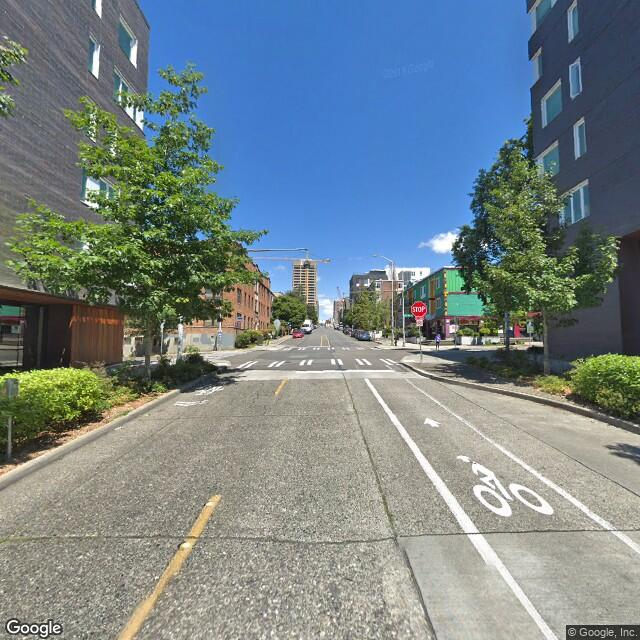
\includegraphics[width=0.4\linewidth]{intro1.jpg}
	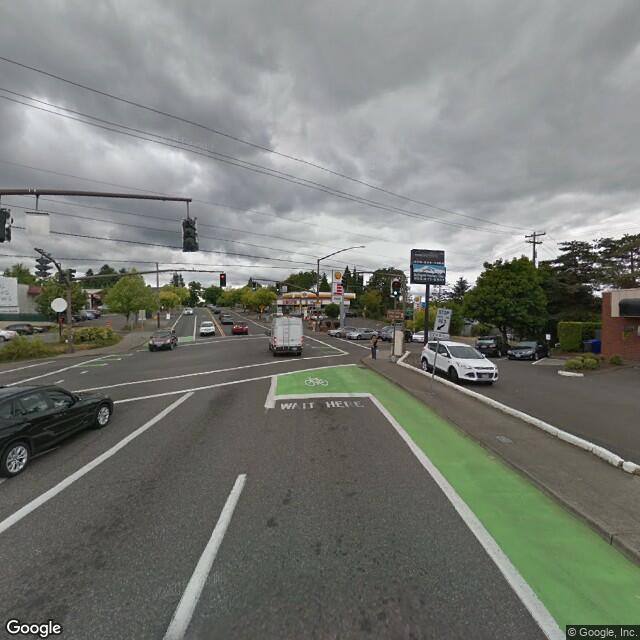
\includegraphics[width=0.4\linewidth]{intro7.jpg}
	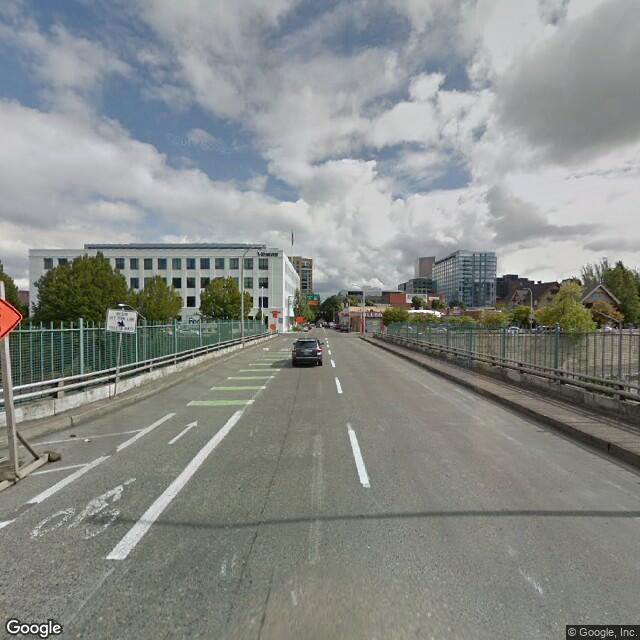
\includegraphics[width=0.4\linewidth]{intro4.jpg}
	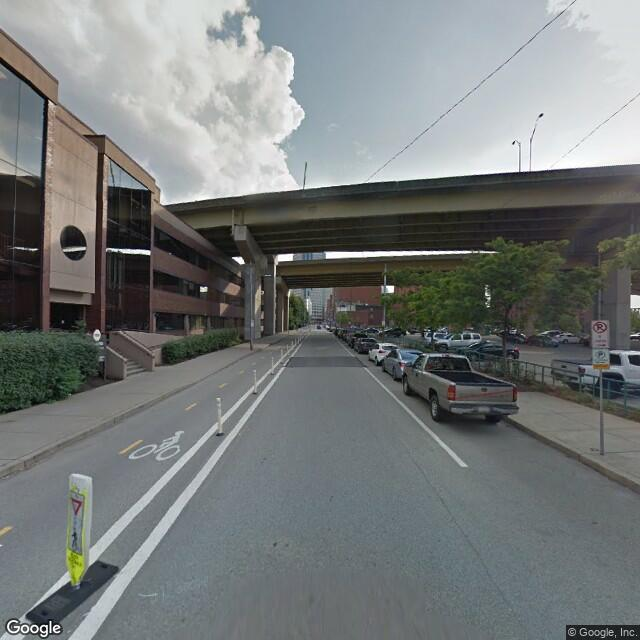
\includegraphics[width=0.4\linewidth]{intro5.jpg}
\end{center}
   \caption{Shared road markings (``sharrows''), colored bike lanes, and barriers are common features of bike-designated roads.}
\label{fig:long}
\label{fig:onecol}
\end{figure}


\begin{figure*}
  \centering
  \subfloat[Bike-designated]{
  	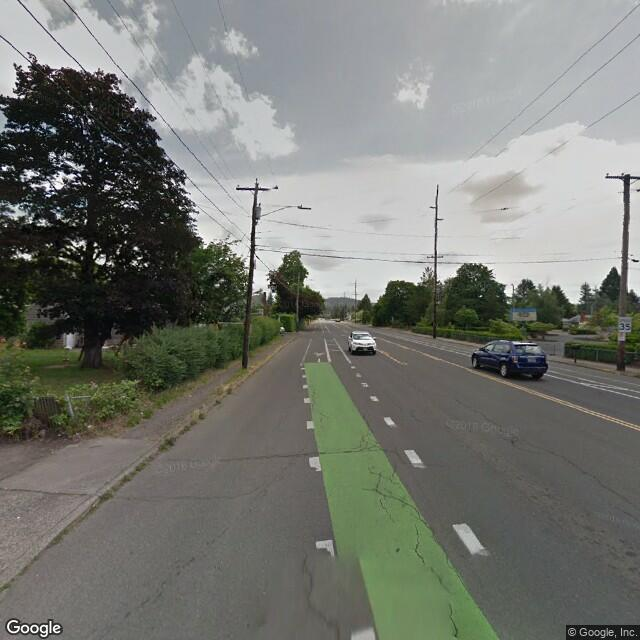
\includegraphics[width=0.1\textwidth]{intro2.jpg}\label{fig:f1}
  	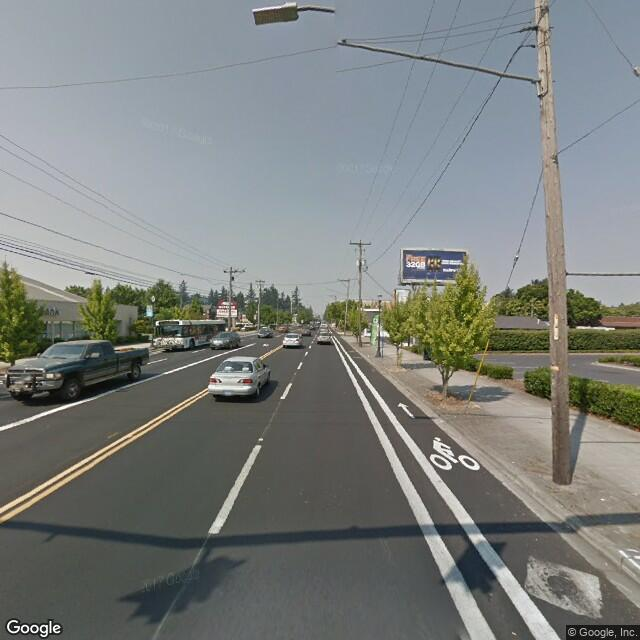
\includegraphics[width=0.1\textwidth]{intro3.jpg}\label{fig:f1}
  	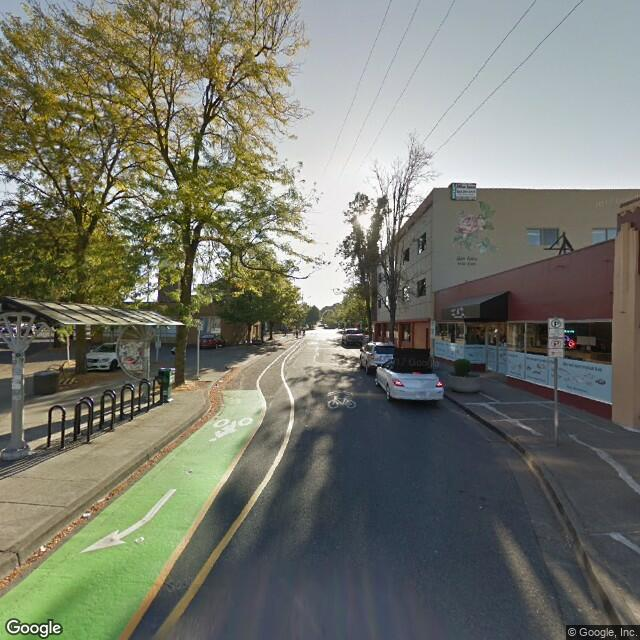
\includegraphics[width=0.1\textwidth]{intro6.jpg}\label{fig:f1}
  	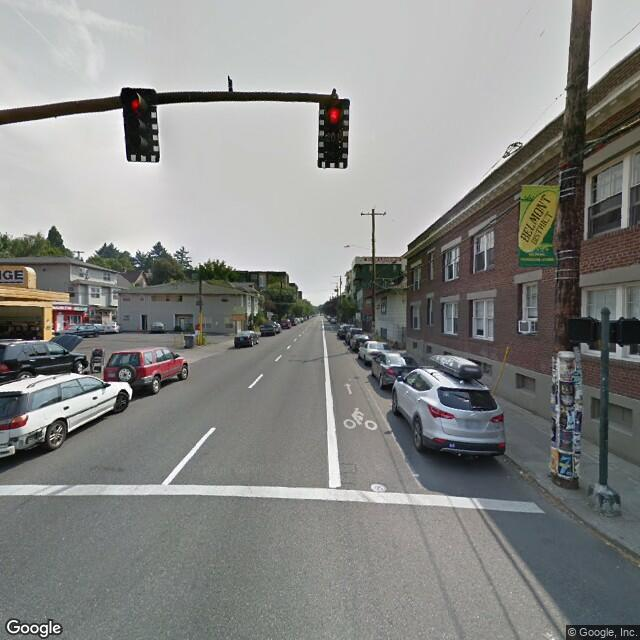
\includegraphics[width=0.1\textwidth]{intro8.jpg}\label{fig:f1}
	}
  \hfill
  \subfloat[Not bike-designated]{
  	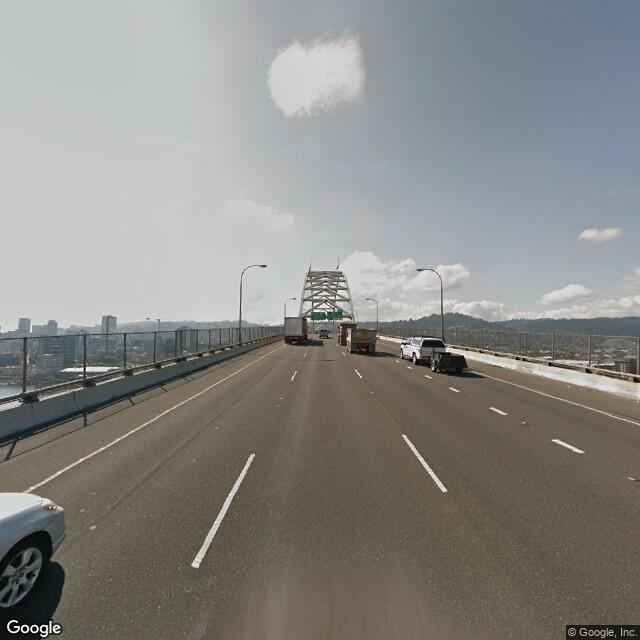
\includegraphics[width=0.1\textwidth]{intro9.jpeg}\label{fig:f1}
  	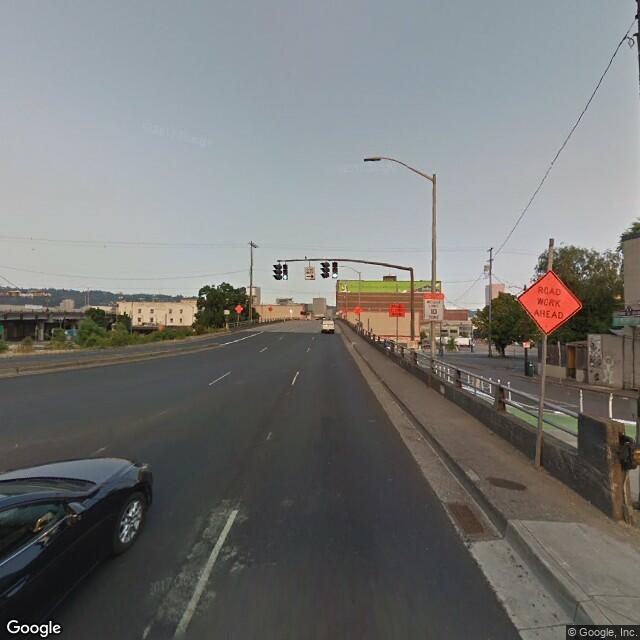
\includegraphics[width=0.1\textwidth]{intro10.jpg}\label{fig:f1}s
  	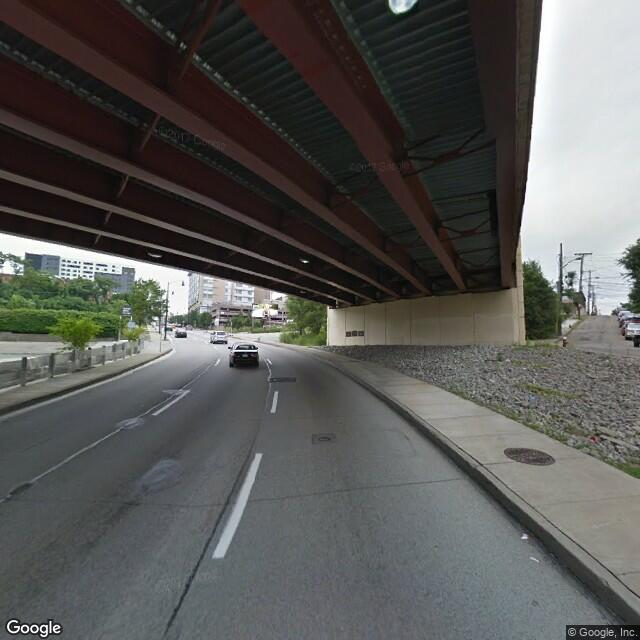
\includegraphics[width=0.1\textwidth]{intro11.jpg}\label{fig:f1}
  	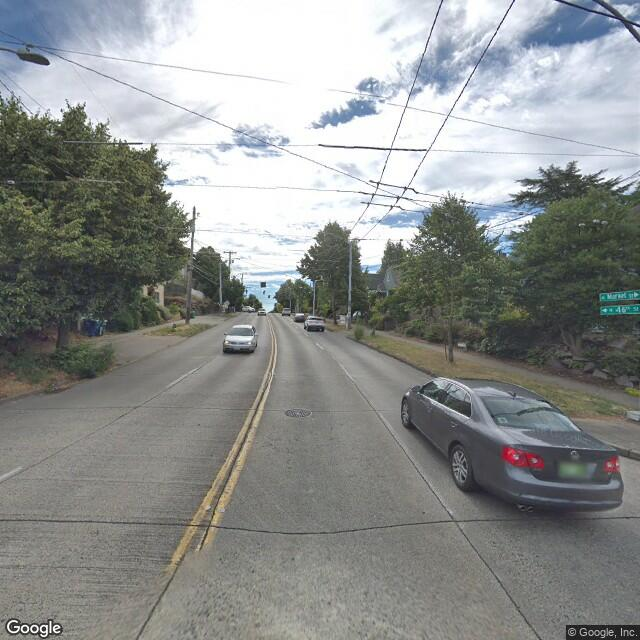
\includegraphics[width=0.1\textwidth]{intro12.jpeg}\label{fig:f1}
  }
  \caption{Example street-view images of bike-designated and not bike-designated roads.}
\end{figure*}

Developing a bike-designation street-view image classifier faces several challenges. First, there is no existing public, large-scale database of street-view images with the bike-designation label. Second, bike-designated roads contain a variety of different types of cycling infrastructure, and each type of infrastructure may look different depending on which city and country the road pertains to. Third, street-view images may not be positioned or oriented correctly to capture the relevant features. Last, street-view images are taken in real-world settings, and face several factors that decrease image quality including feature occlusion, background clutter, differences in illumination, and blur.

To overcome the first challenge, we generate a labeled dataset of street-view images by integrating OpenStreetMap road classification data with Google's Street View API. To overcome the remaining challenges, we develop a convolutional neural network to classify street-view images as bike-designated or not. Previous research has demonstrated the effectiveness of CNNs for scene understanding and object detection in real-world settings, where viewpoint variation, occlusion, background clutter, illumination, and intra-class variation are expected [cite 231]. 

The paper is structured as follows. Section \ref{sec:background} presents related research. Section \ref{sec:approach} explains our approach to developing a labeled dataset, neural network, and human baseline. Section \ref{sec:experiments} contains the results of our experiments to improve our network's performance. Section \ref{sec:conclusion} concludes with lessons learned and directions for future research.

%%%%%%%%% RELATED WORK
\section{Background and Related Work}
\label{sec:background}

\subsection{Scene Classification}
Convolutional neural networks have been widely successful in object classification tasks \cite{krizhevsky2012imagenet}. Trained on massive datasets, these networks have been able to nearly achieve or even exceed human performance benchmarks.

Scene classification, however, is a more challenging, generalized task than object classification: a scene class may be correlated with the presence of objects, but such objects may appear in other scene classes. Correctly classifying a scene depends not only on objects but also attributes (relating to spatial envelope, materials, lighting, and textures).

Xiao et al. developed the SUN Database, the first large-scale scene understanding database with 899 scene categories and over 130,000 labeled images\cite{xiao2010sun}. Shortly thereafter, Patternson and Hays developed the first large-scale scene attributes dataset and demonstrate the predictive power of attributes for classifying scenes \cite{6247998}. Most recently, Zhou et al. develop the Places database, a database of 434 scene categories and over 10 million scene images \cite{DBLP:journals/corr/ZhouKLTO16}. Using the Places database, Zhou et al. surpassed previous scene classification benchmarks using VGG, GoogLeNet, AlexNet, and ResNet convolutional neural networks. 

\subsection{Street View Images}
Several researchers have used Google Street View images as a source of natural images; Google Street View cars take panoramic photos along roads, providing a rich source of images of outdoor scenes. Netzer et al use Street View images to generate the Street View House Number dataset for digit classification. Similarly, Slavkovikj et al. use Street View images to develop a road-texture dataset for classification [cite]. Gebru et al. develop a car brand classifier [cite], and Hershey and Wulfe use deep learning to recognize geo-location from city Street View images.

%%%%%%%%% APPROACH
\section{Approach}
\label{sec:approach}


\subsection{Data}
To generate a labeled dataset of bike-designated street-view images, we created a tool to integrate OpenStreetMap road classifications with Google's Street View API. This tool does the following:
\begin{enumerate}
\item Download OpenStreetMap data for a particular region
\item Extract road segments (way elements) for this region using particular criteria
\item Extract road points (node elements) for these ways using particular criteria
\item Calculate road orientation for each for these nodes
\item Query Google's Street View API using node coordinates and road orientation
\item Save the street-view image with the road classifications
\end{enumerate}
Specifically, to create a dataset of bike-designated images, we did the following.

In step 1, we used OpenStreetMap data for four cities: Boulder, Pittsburgh, Portland, and Seattle. We chose these regions because of the quality and availability of bike-designation for roads in these cities, and because these cities have near-balance between bike-designated and non-designated roads (in total, 57\% and 43\%).

In step 2, we filtered road segments to only include road types ``motorway'', ``primary highway'', ``secondary highway'', and ``tertiary highway''. Other segment types included non-road segments not relevant to our analysis such as footpaths and bike-paths, as well as residential roads, which were often unlabeled with road classifications.

In step 3, we filtered nodes to only include the midpoint of each road. Given the cost of the Google Street View API (\$7 per 1000 images), we could not capture Street View images at all millions of nodes of all relevant highways. Nodes are typically several meters apart; so, capturing Street View images at adjacent nodes will result in similar images with a slightly shifted camera perspective. Extracting a single image for each road segment (rather than extracting multiple images at a subset of road segments) increases image heterogeneity while keeping our API costs reasonable.

In step 4, we determine the required camera orientation such that each image is pointed in the direction of the road. To do so, we calculate the geodesic azimuth (angular distance from north) between a node and the subsequent node. For one-way roads, we orient the camera to face in the forward-direction of the road.

In step 5, we query the API to determine if a Street View image is available for the given coordinate in a radius of 10 meters. We found that reducing the search radius to 10 meters decreased the chance that images of nearby (but different) roads were not accidentally downloaded in the case that a road did not have street-view images. Then, if an image is available, we download a 640x640 image using the node coordinate and the calculated camera orientation.

\subsection{Neural Network}
To classify images as bicycle friendly or not, we relied on convolutional neural network architectures to predict the label of our input data. More specifically, the type of convolutional neural network that we tested was a residual neural network (ResNet) [?], which has “shortcut connections” that skip one or more convolutional layers to make training of deeper networks more efficient. In general, training CNNs can be time consuming and computationally expensive. To avoid training an entire ResNet, we decided to apply the knowledge transfer method known as transfer learning[?].

Transfer learning is a method that can speed up the training process of building a neural network architecture by a great factor. The idea behind this method is to find a pre-existing network architecture that has already been trained for a similar problem, and apply the information that this pre-trained network has learned for a different problem. With the pretrained information, the next training step is to ‘fine-tune’ the network, or tweak the model in a way that is more practical for the other problem. We chose this training method not only for its time saving benefits, but also for the ability to effectively train models.

We researched numerous different architectures that were modelled for a similar type of classification. In our case, we used the weights from a pretrained ResNet18 model that was trained on the Places365 dataset [?], which is an image dataset that is used for recognition of scenes (ie. different indoor/outdoor environments). This model was useful for transfer learning because the convolutional layers have already learned low level features such as lines, edges, shapes that make up attributes of different indoor/outdoor environments.

We downloaded the pre-trained architecture of this model and ‘froze’ the convolutional layers. This means that we set the weights of the convolutional layers to not be affected by gradient descent. With the convolutional layers frozen, we chopped off the final fully-connected layer that came with the model and added layers at the end of the model to fine-tune the model to our specific classification problem. The experiments that we ran for this are further discussed in section [].  The final architecture of our network can be seen in Figure 3. 

why we chose pre-trained places365, why we chose to fine-tune, how we came up with the final model
pictures of training/val loss accuracy

\begin{figure}[t]
\begin{center}
	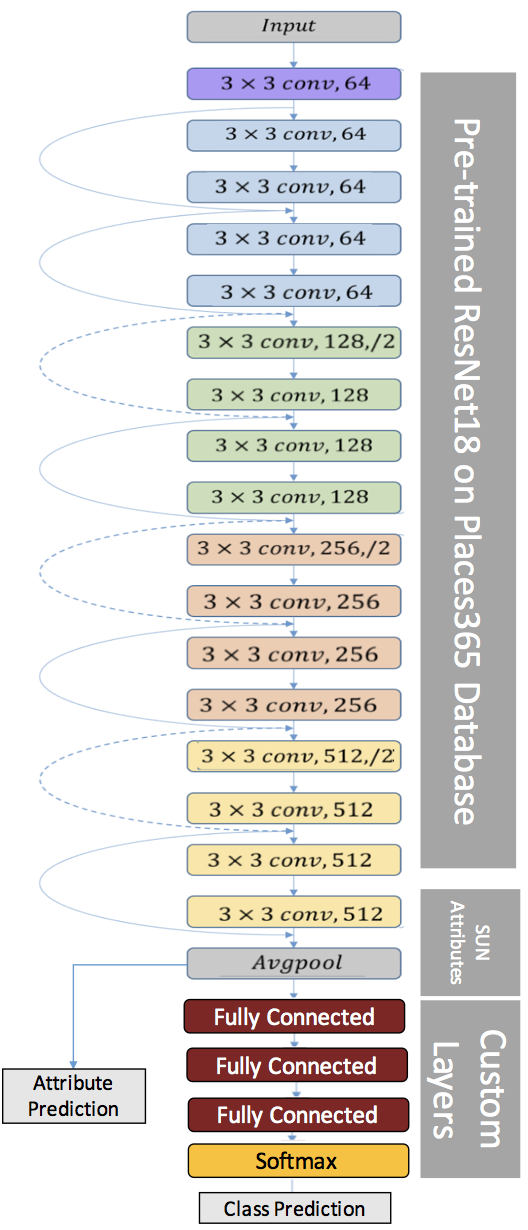
\includegraphics[width=.75\linewidth]{model.png}
\end{center}
	\caption{Final model: Pre-trained ResNet18 with three fine-tuned fully-connected layers.}
\label{fig:long}
\label{fig:onecol}
\end{figure}

\subsection{Human Benchmark}
We noticed while going through our dataset that classifying a road as bicycle friendly or not could potentially be a difficult classification task even for humans. We hypothesized that if we give our test images to humans, then our network would out perform a human baseline. 

To test this theory, we built a user interface that allowed humans to predict the label of a randomly selected test image. The user interface included a random test image and two buttons that the user could press which submitted their prediction as ‘bike friendly’ or ‘not bike friendly’. Once pressed, a new randomly selected test image would be loaded and the user can predict once more. The human The user interface for this demonstration can be seen in Figure []. 

A number of UMass students volunteered to participate in our experiment to create a human baseline for this classification problem. Overall, we had 17 participants that ran experiments. On average, each participant made predictions on 77 images. In total, people made predictions on 1,313 images with a total accuracy of 59.5\%. 


\begin{figure}[t]
\begin{center}
	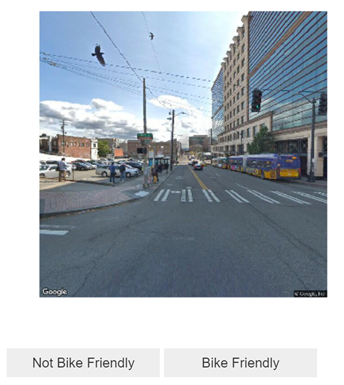
\includegraphics[width=.7\linewidth]{gui.png}
\end{center}
	\caption{The Human Benchmark test user interface.}
\label{fig:long}
\label{fig:onecol}
\end{figure}

%%%%%%%%% EXPERIMENTS
\section{Experiments}
\label{sec:experiments}

To ensure that our final model would perform well, we trained a wide variety of models on our dataset. We combined a number of different models with a variety of hyperparameter values to see how they learn to our dataset. With a collection of model performances, we selected the best performing ones to be trained on the entire dataset.

We started off by sampling the training and validation data even further so that we had small batches of training and validation data (approximately 10\% of the entire training/validation set). Having smaller batches of the training data allowed us to efficiently train more models in a reasonable amount time. 

We then experimented with a number of different models and hyperparameters on our sampled training/validation set. All of the models were built off the 'head' of the frozen convolution layers. The different types of models that were trained include, 1 to 3 fully connected layers, with and without dropout and the Leaky ReLU activation function.

Along with these various models, a number of different hyperparameters were tested. These models were trained with a variety of optimizers, regularization strengths and hidden layer sizes. The optimizers that were considered for our network architectures in Adam and Stochastic Gradient Descent (SGD) with momentum. 

Each of these models were combined with the various hyperparameters to see how well they learned the input data. Each of the models were trained on the sample training data set and then tested on the the sampled validation set. To see how well the models performed, we plotted the all of the models accuracy curves over a number of epochs. We analyzed the accuracy plots of each of the models to see how they respond to the training data. 

From our analysis, we found a number of models would overfit to the training data. Other models would not learn any features and would have accuracies that would be equivalent to random guesses. Some models seemed to learn to the data and not overfit. Further analysis of the training/validation accuracy curves, lead us to choose the final model. The final model has 3 fully connected layers, with 10\% dropout in between each layer, softmax at the end, SGD with momentum optimization, learning rate of 0.1, and a hidden layer size of 400. We found that this model did not overfit to the training data and was able to learn features of the input data over time while minimizing loss. 

\begin{table}[t]
\begin{center}
	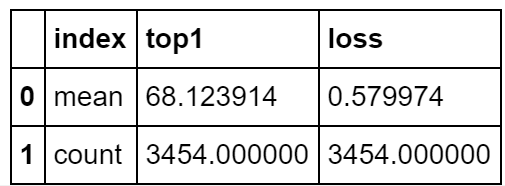
\includegraphics[width=0.7\linewidth]{final_acc_table.png}
\end{center}
   \caption{Test accuracy \& loss for the final model.}
\label{fig:long}
\label{fig:onecol}
\end{table}

\begin{table}[t]
\begin{center}
	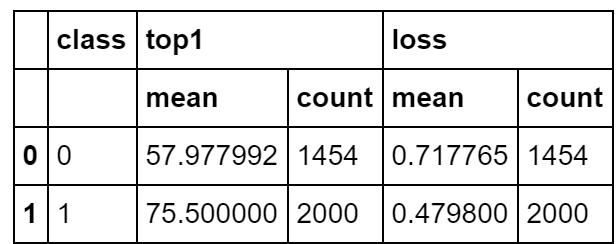
\includegraphics[width=0.7\linewidth]{final_acc_by_label_table.png}
\end{center}
   \caption{Test accuracy \& loss for each class label in the final model.}
\label{tab:long}
\label{fig:onecol}
\end{table}

We took all of the hyperparameters of the best performing model created the 'final model' seen in Figure [?]. We trained the final model on the full training set (60\% of the entire dataset). The results of training the model on the entire training dataset can be seen plotted in the training/validation accuracy curve plotted in Figure []. With the model fully trained, we ran it on our test set (20\% of the entire dataset). The results from the test set showed that our model had an overall accuracy of \textbf{68.12\%}, seen in Table 1. Since this is a binary classification task, it is important to look at the \textit{per-label accuracy}. We found that the model was able to make successful predictions for the non-bike friendly class \textbf{57.97\%} of the time, and \textbf{75.5\%} of the time for the bike-friendly class, the results can be seen in Table 2. 

% different models: fc1, fc2, fc3, w/wout dropout, leakyrelu
% different optimizers: adam, SGD with momentum + L2 reg
% hyperparameter search: learning rate, reg strength, hidden layer size
% how we chose: trained on 10\% of dataset, looked at loss/acc curves

% show images, CAM, attributes, with our prediction
% top accuracy for our models (68\%)

% final model: fc3 (400 units?), 10\% dropout and leakyrelu, SGD + momentum, L2 reg

% This section begins with what kind of experiments you're doing, what kind of dataset(s) you're using, and what is the way you measure or evaluate your results. It then shows in details the results of your experiments. By details, we mean both quantitative evaluations (show numbers, figures, tables, etc) as well as qualitative results (show images, example results, etc).


\begin{figure}[t]
\begin{center}
	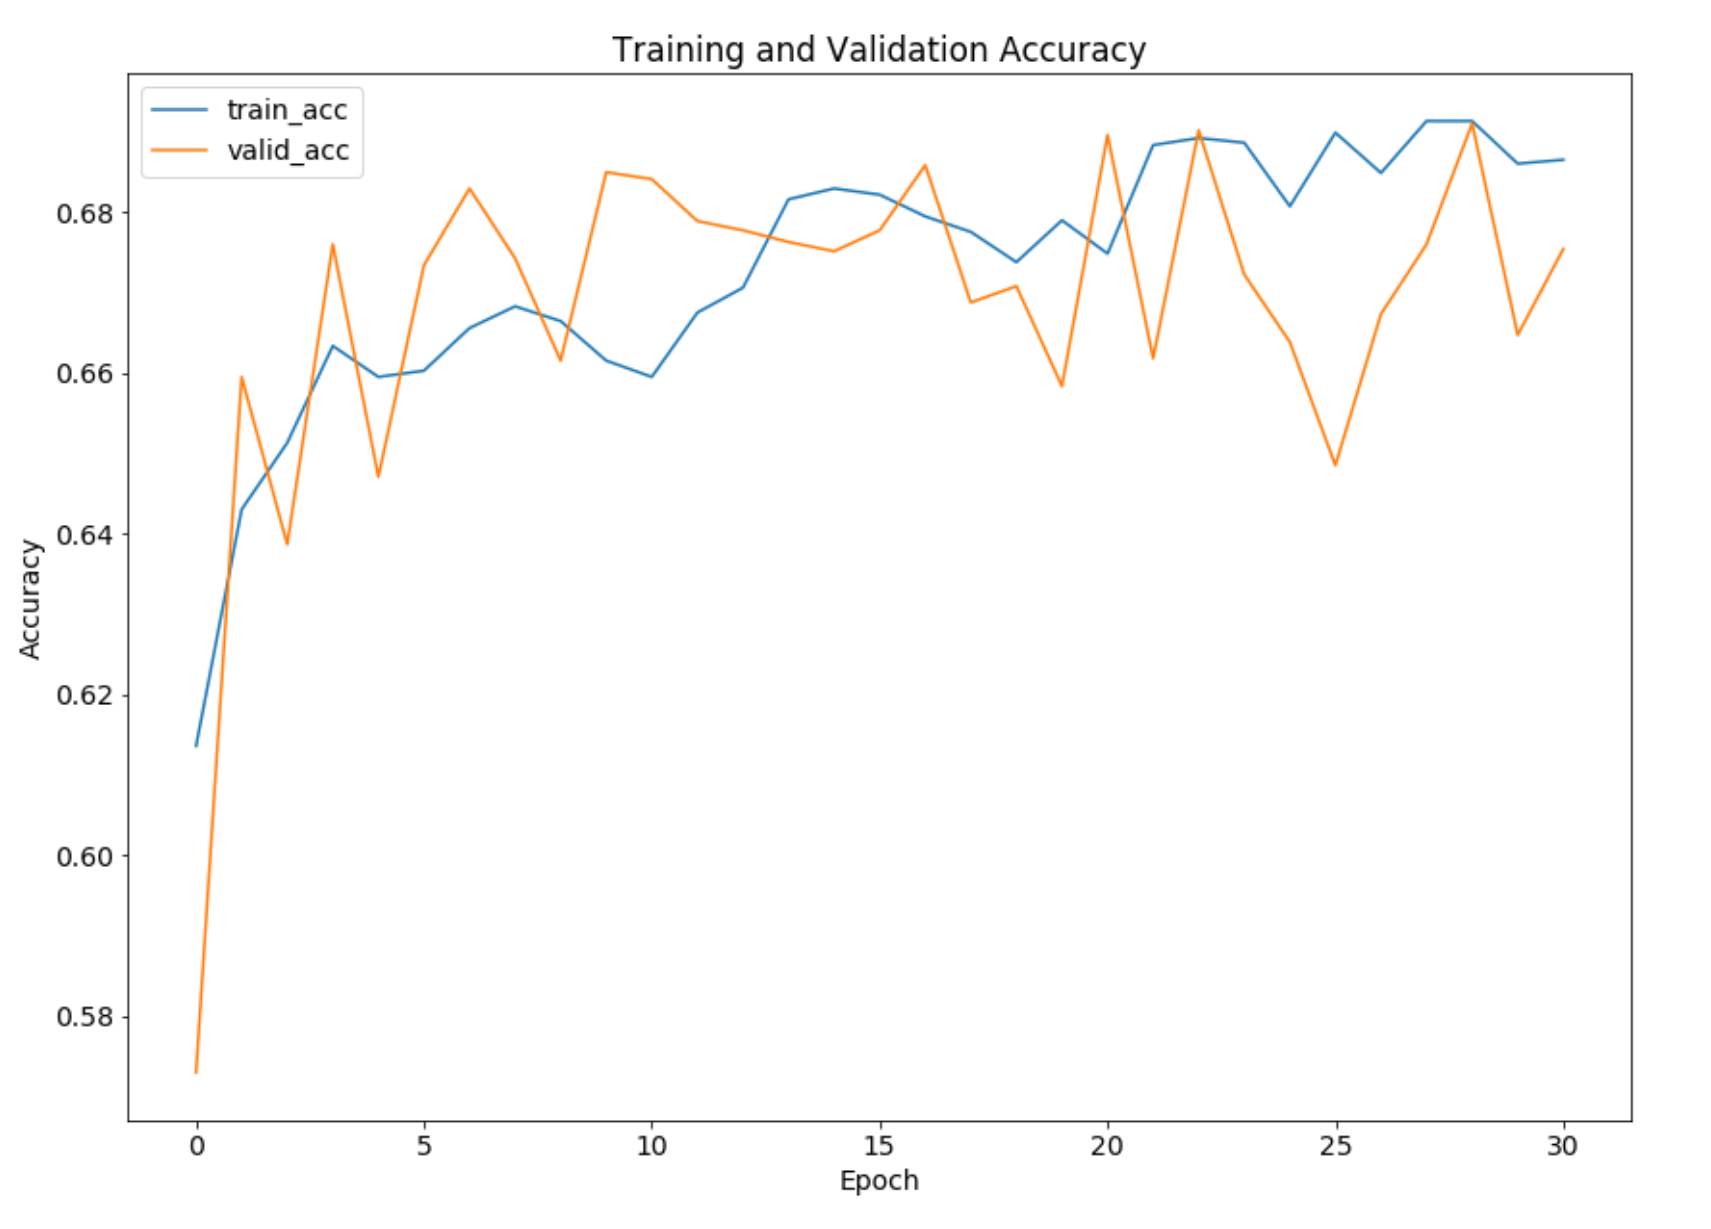
\includegraphics[width=1\linewidth]{final_acc_curve.png}
\end{center}
   \caption{Training \& Validation accuracy curve for the final model.}
\label{fig:long}
\label{fig:onecol}
\end{figure}


A useful feature of this model architecture is  to be able to extract attributes from the input data and to also generate Class Activation Maps (CAM). From the last convolution layer of the ResNet18, attributes are extracted from the features that the model can recognize in the input data. These attributes are from the SUN attributes dataset [?] which describes images with a set of attributes.  Using the weights of the classes, we are able to generate a CAM of an image to visualize what features of the image are responsible for the models prediction. The attributes along with a CAM can be seen in Figure []. Using these attributes and maps, we can qualitatively determine the difficulty of predicting one class over the other.



\begin{figure}[t]
\begin{center}
	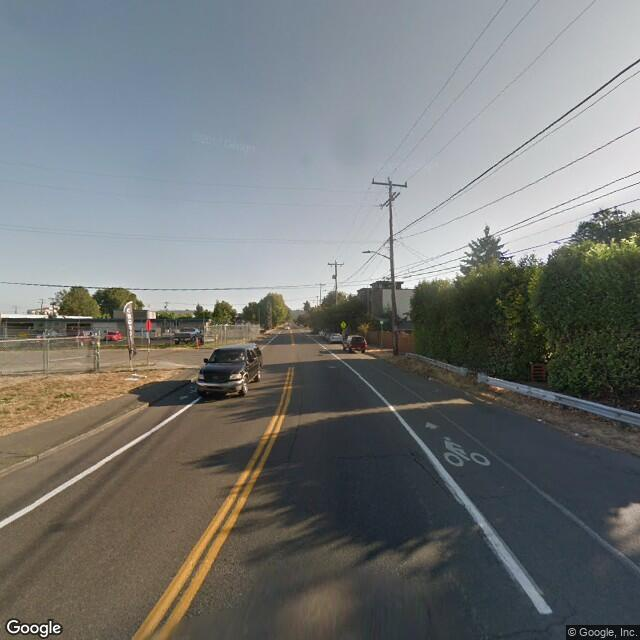
\includegraphics[width=0.4\linewidth]{bf.jpg} 
	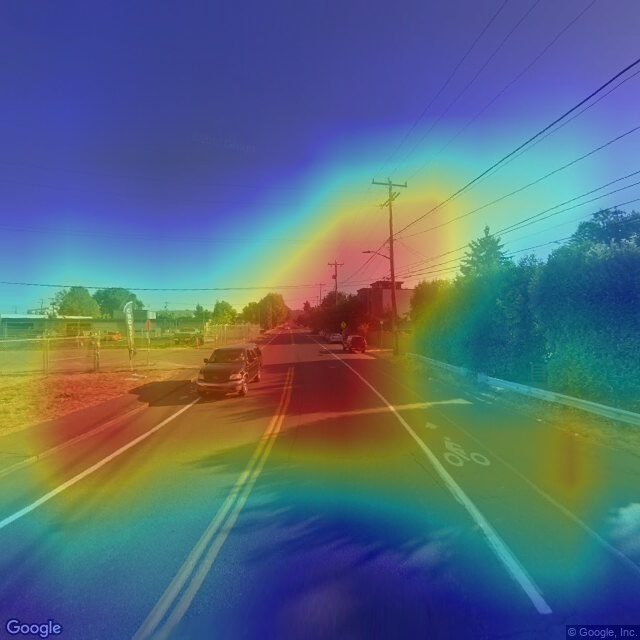
\includegraphics[width=0.4\linewidth]{bf_cam.jpg} 

Top Attributes:
open area, natural light, man-made, asphalt, driving, biking, far-away horizon, transporting, sunny

	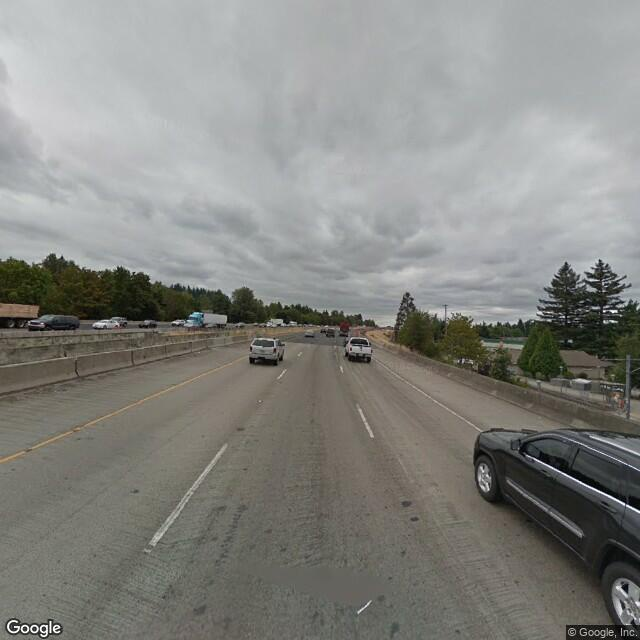
\includegraphics[width=0.4\linewidth]{non_bf.jpg}
	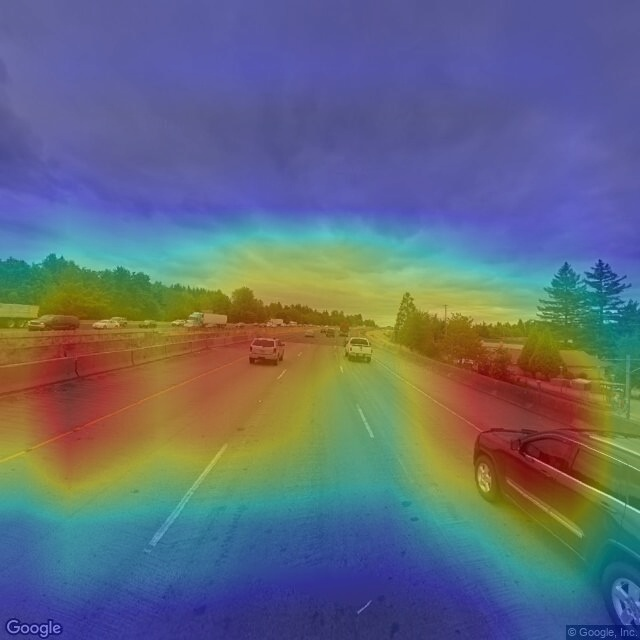
\includegraphics[width=0.4\linewidth]{non_bf_cam.jpg}

Top Attributes:
open area, natural light, man-made, far-away horizon, driving, clouds, asphalt, transporting, biking

\end{center}
   \caption{Bicycle friendly road alongside its Class Activation Map (CAM), top. Non-Bicycle-friendly road alongside CAM, bottom.}
\label{fig:long}
\label{fig:onecol}
\end{figure}







%%%%%%%%% CONCLUSION
\section{Conclusion}
\label{sec:conclusion}
What have you learned? 

Suggest future ideas.\\

List and number all bibliographical references at the end of your paper. When referenced in the text,
enclose the citation number in square brackets, for
example. \\

TODO: add the rest of the citations here from cs682\_final\_report.bib

\cite{slavkovikj2014image}
\cite{patterson2014sun}
\cite{rundle2011using}
\cite{zhou2017places}
\cite{DBLP:journals/corr/ZhouKLOT14}
\cite{DBLP:journals/corr/Wang15l}
\cite{DBLP:journals/corr/HeZRS15}
\cite{DBLP:journals/corr/ZagoruykoK16}
\cite{DBLP:journals/corr/ZhouKLTO16}
\cite{koehrsen2018blog}

{\small
\bibliographystyle{ieee}
\bibliography{cs682_final_report.bib}
}

\end{document}
